\documentclass[12pt,a4paper,openright]{book}

% =======================
% Pacotes básicos
% =======================
\usepackage[utf8]{inputenc}
\usepackage[T1]{fontenc}
\usepackage[brazil]{babel}
\usepackage{geometry}
\geometry{a4paper, top=2.5cm, bottom=2.5cm, left=2.5cm, right=2.5cm}
\usepackage{float}
\usepackage{graphicx}    % Para inserir logo/imagens
\usepackage{xcolor}      % Cores
\usepackage{hyperref}    % Links clicáveis
\usepackage{minted}      % Código com destaque (compilar com -shell-escape)
\usepackage{tcolorbox}   % Caixas estilizadas
\usepackage{titlesec}    % Para customizar títulos
\usepackage{fancyhdr}    % Cabeçalho e rodapé
\usepackage{tikz}        % Para desenhar capa com moldura colorida
\usepackage{caption}
\usepackage{amsmath}
\usepackage{amsfonts} 
\usepackage{amssymb}
% =======================
% Cores personalizadas
% =======================
\definecolor{verdeuni}{RGB}{0,70,40} % Verde do logo UniRV
\definecolor{bgsql}{rgb}{0.95,0.95,0.95}
% FIX: Para o erro do fancyhdr headheight
\setlength{\headheight}{26pt} 
\addtolength{\topmargin}{-1.5pt}
% =======================
% Cabeçalho e rodapé
% =======================
% --- Configuração de Cabeçalho e Rodapé ---
\pagestyle{fancy}
\fancyhf{}

% Nome do autor no lado esquerdo
\lhead{\color{verdeuni} \textbf{Prof. Me. Sergio Souza Novak}} 

% Título do guia no lado direito
\rhead{\textbf{\color{verdeuni}Lógica para Engenharia de Software}}

% Número da página no centro do rodapé
\cfoot{\thepage}

% Linha horizontal colorida (opcional, combina com o estilo)
\renewcommand{\headrulewidth}{0.4pt}
\renewcommand{\headrule}{\hbox to\headwidth{\color{verdeuni}\leaders\hrule height \headrulewidth\hfill}}

% =======================
% Sumário automático
% =======================
\setcounter{tocdepth}{2} % mostra até subseções
\hypersetup{
    colorlinks=true,
    linkcolor=verdeuni,
    urlcolor=blue 
}

% =======================
% Estilo de títulos
% =======================
\titleformat{\section}{\Large\bfseries\color{black}}{\thesection}{1em}{} % seções em preto
\titleformat{\subsection}{\large\bfseries\color{verdeuni}}{\thesubsection}{1em}{} % subseções no verde

% =======================
% Caixa para exemplos de SQL
% =======================
\tcbuselibrary{minted}

\newtcblisting{sqlcode}{
    listing engine=minted,
    minted language=sql,
    colback=bgsql,
    colframe=verdeuni,
    listing only,               % só mostra código
    title=SQL,                  % título visível
    fonttitle=\bfseries\color{white},
    coltitle=white,
    colbacktitle=verdeuni
}

\newtcolorbox{diagramER}{
    colback=white,
    colframe=verdeuni,
    title=Diagrama ER,
    fonttitle=\bfseries\color{white},
    coltitle=white,
    colbacktitle=verdeuni,
    boxrule=0.8pt,
    arc=2mm,
    left=4mm,
    right=4mm,
    top=3mm,
    bottom=3mm
}
  
% =======================
% Caixa para observações
% =======================
\newtcolorbox{observacao}{
    colback=green!5,
    colframe=verdeuni,
    boxrule=0.6mm,
    arc=2mm,
    left=4mm,
    right=4mm,
    top=3mm,
    bottom=3mm
}
% =======================
% Definição dos Blocos (FIX para o erro de Environment undefined)
% =======================
\newtcolorbox{block}[1]{%
  colback=green!5,
  colframe=verdeuni,
  coltitle=white,
  title=#1,
  fonttitle=\bfseries,
  boxrule=1pt,
  arc=2mm,
  left=6pt,
  right=6pt,
  top=6pt,
  bottom=6pt
}
% =======================
% Dados do documento
% =======================
\title{Lógica para Engenharia de Software}
\author{Me. Sergio Souza Novak}
\date{\today}
% =======================
% Página de Apresentação do Autor
% =======================
\newcommand{\authorpage}{
  \newpage
  \thispagestyle{empty} % sem cabeçalho e rodapé
  \begin{tikzpicture}[remember picture, overlay]
    % Fundo verde escuro
    \fill[verdeuni] (current page.north west) rectangle (current page.south east);
  \end{tikzpicture}

  \begin{center}
        {\color{white}\bfseries\LARGE Me. Sergio Souza Novak, autor deste livro.}
    \vspace{1cm}

    % Foto do autor
    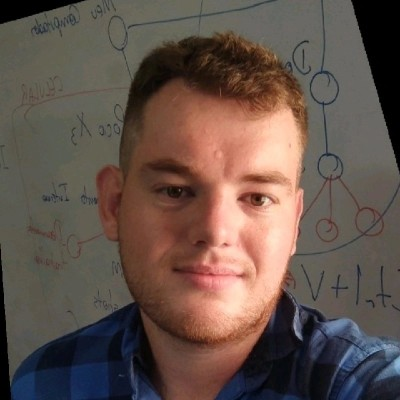
\includegraphics[width=5cm,height=5cm,keepaspectratio]{foto_sergio.jpeg} % coloque o nome do arquivo da sua foto

    \vspace{1cm}
    % Texto da biografia
    \begin{minipage}{0.85\textwidth}
      \color{white} % texto branco para contraste com o fundo verde escuro
      \small
      Sergio Souza Novak, nascido em 7 de dezembro de 1996 em Corbélia (PR),
      iniciou o curso de Ciência da Computação na UNIOESTE em 2017, onde também atuou
      como professor de apoio a pessoas com necessidades especiais, especialmente à
      comunidade surda, nas áreas de Programação, Física e Matemática. Filho de Sergio
      Novak, mecânico, e Rosilei de Souza Novak, doutora pela Universidade Federal do
      Paraná (UFPR), mudou-se com a família para Rio Verde (GO) em 2018. Nesse mesmo
      ano transferiu-se para o Instituto Federal Goiano (IF Goiano) para dar continuidade à
      graduação, período em que também lecionou cursos de Informática na Prefeitura
      Municipal de Rio Verde. Além de ministrar cursos na prefeitura, ainda ministrou aulas
      em 2019 no Programa Nacional de Acesso ao Ensino Técnico e Emprego (PRONATEC),
      do Governo Federal, para o curso de Redes de Computadores e Programação de Jogos Digitais. 
      Tendo se formado em Bacharelado em Ciência da Computação, em 2022, trabalhou como
      Desenvolvedor de Software em uma empresa de Belo Horizonte, Minas Gerais, chamada 
      Engenharia Assistida por Computador (ENACOM), concomitantemente com a rotina de professor. 
      Atuou como desenvolvedor, construindo sites por mais de dois anos na ENACOM, produtos voltados
      à otimização de processos industriais, siderurgia e logística. Durante a pandemia de COVID-19 desenvolveu pesquisas e
      trabalhos sobre o funcionalismo público e e, graças a parcerias com
      pesquisadores do IF Goiano, rendendo então, publicações na área da Gestão Pública.
      Ingressou em 2024 no Programa de Pós Graduação em Ciências Agrárias (PPGCA-AGRO),
      nível mestrado, do Instituto Federal Goiano. Durante o mestrado, no Laboratório de Irrigação
      do Instituto Federal Goiano, desenvolveu mais de dez (10) programas de computador registrados no Instituto Nacional
      da Propriedade Industrial (INPI) e diversos artigos na área de Inteligência Artificial. No IF Goiano atuou em projetos
      em outros programas de pós-graduação. Em parceria com a Pós-graduação em Biodiversidade e
      Conservação (PPGBio), publicou trabalhos em Inteligência Artificial para detecção de Abelhas Nativas
      do Cerrado e também na fruticultura e psicultura. Atualmente, Sergio é Mestre em Ciências Agrárias e professor na Universidade de Rio Verde (UNIRV), docente responsável pela disciplina de Lógica para Engenharia de Software no curso de Engenharia de Software.
    \end{minipage}
  \end{center}
  \newpage
}
% =======================
% Capa Estilo Tanenbaum
% =======================
\newcommand{\makecapa}{
  \begin{titlepage}
    \thispagestyle{empty}

    \begin{tikzpicture}[remember picture, overlay]
      % Faixa Superior (Topo) - Cor Verdeuni
      \fill[verdeuni] (current page.north west) rectangle ++(\paperwidth,-6.5cm);
      
      % Texto do Topo: Autores e Título Principal
      \node[anchor=north, text width=\paperwidth, align=center] at ([yshift=-1.5cm]current page.north) {
        {\Large\sffamily\color{white}  ME. SERGIO SOUZA NOVAK } \\[0.8cm]
        {\Huge\bfseries\sffamily\color{yellow} Lógica para Engenharia de Software} \\[0.4cm]
        {\Large\sffamily\color{white} 1ª EDIÇÃO}
      };

      % Imagem Central (A ilustração de commodities que geramos)
      % Ela fica posicionada entre as faixas, como no livro original
      \node[anchor=center] at ([yshift=-2.2cm]current page.center) {
        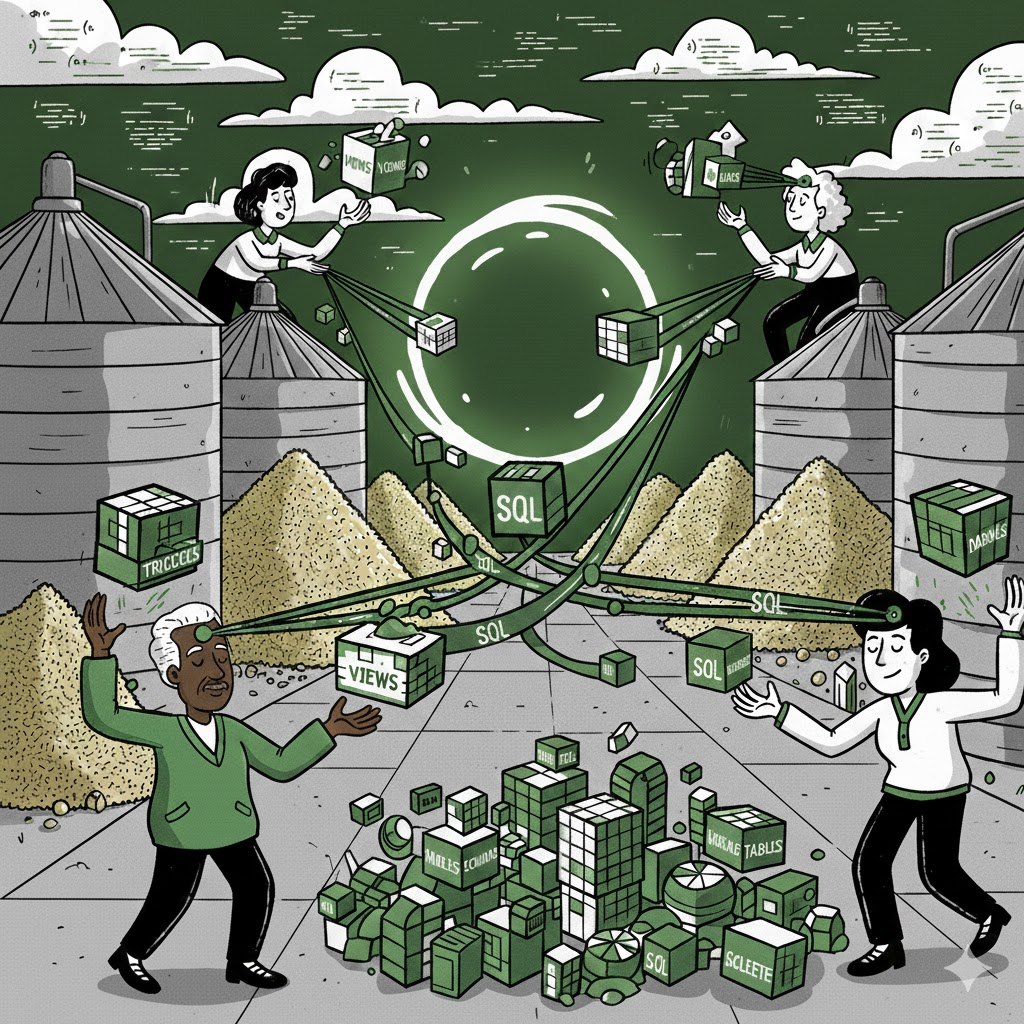
\includegraphics[width=1.02\paperwidth]{capa.jpg} % Ligeiramente maior para sangria lateral
      };

      % Faixa Inferior (Rodapé) - Cor Verdeuni
      \fill[verdeuni] (current page.south west) rectangle ++(\paperwidth,2cm);
      
      % Texto do Rodapé: Instituição e Data
      \node[anchor=south, text width=\paperwidth, align=center] at ([yshift=0.7cm]current page.south) {
        % {\large\sffamily\color{white} \textbf{UNIVERSIDADE DE RIO VERDE} \quad | \quad \today}
      }; 
      
      % Detalhe branco no rodapé (simulando o "Pearson" ou "Always Learning")
      \node[anchor=south east, xshift=-1cm, yshift=0.6cm] at (current page.south east) {
        % {\small\sffamily\color{white} UniRV}
      };
    \end{tikzpicture}

  \end{titlepage}
}

% =======================
% Capa personalizada
% =======================
\newcommand{\maketitlecustom}{
  \begin{titlepage}
    \thispagestyle{empty}
    % Moldura verde escura em cima e embaixo
    \begin{tikzpicture}[remember picture, overlay]
      % Cabeçalho verde
      \fill[verdeuni] (current page.north west) rectangle ++(\paperwidth,-2cm);
      % Rodapé verde
      \fill[verdeuni] (current page.south west) rectangle ++(\paperwidth,2cm);
    \end{tikzpicture}

    % Conteúdo centralizado na página
    \vspace*{3cm}
    \begin{center}
      % Logo central grande
\setlength{\fboxrule}{1pt}
      \fbox{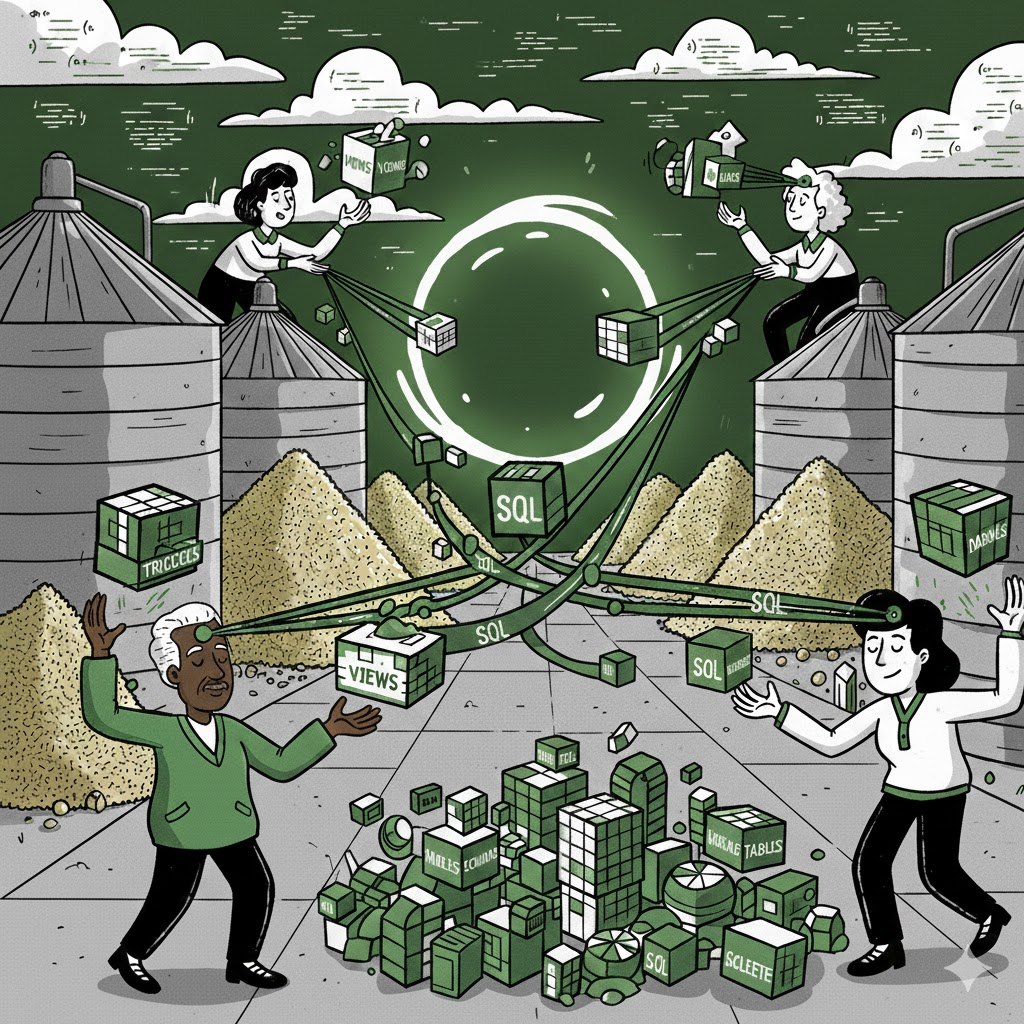
\includegraphics[width= 10cm ]{capa.jpg}}


      \vspace{1.5cm}
      {\Huge\bfseries\color{verdeuni} Capítulo 1 - Conhecendo as ferramentas}

      \vspace{1cm}
      {\Large Universidade de Rio Verde}

    \end{center}

  \end{titlepage}
}

% =======================
% Documento
% =======================
\begin{document}

% Capa personalizada
\makecapa

% \maketitlecustom
\authorpage

% Sumário
\tableofcontents

% =======================
% Conteúdo convertido dos slides
% =======================

\chapter{Introdução e Contexto Histórico}
\section{Pierre de Fermat (1607–1665)}

\begin{block}{Quem foi Fermat?}
Pierre de Fermat foi um matemático francês do século XVII, reconhecido como um dos principais responsáveis pelo desenvolvimento da Teoria dos Números moderna. Embora tenha exercido profissionalmente a carreira de jurista e magistrado, suas contribuições matemáticas foram profundas e influenciaram gerações de pesquisadores.
\end{block}

Pierre de Fermat nasceu em Beaumont-de-Lomagne, no sul da França, em 1607. Formou-se em Direito e atuou como conselheiro no Parlamento de Toulouse, cargo que ocupou durante grande parte de sua vida. Diferentemente de muitos matemáticos de sua época, Fermat não era professor universitário nem publicava sistematicamente seus trabalhos. Ele desenvolvia a Matemática por interesse pessoal, dedicando-se a ela como uma atividade intelectual paralela à sua carreira jurídica.

Grande parte de suas descobertas foi registrada em cartas trocadas com outros estudiosos e em anotações escritas nas margens de livros que estudava. Esse hábito peculiar contribuiu para a aura de mistério que envolve sua obra.

\section{Provas nas Margens dos Livros}

\begin{block}{Um hábito que marcou a história da Matemática}
Fermat costumava registrar teoremas e resultados matemáticos nas margens de suas cópias de obras clássicas, frequentemente sem apresentar demonstrações completas.
\end{block}

Seu estilo conciso e, por vezes, enigmático, desafiou matemáticos posteriores a demonstrar rigorosamente suas afirmações. A mais famosa dessas anotações ficou conhecida como o \textit{Último Teorema de Fermat}. Ao estudar uma edição da obra \textit{Arithmetica}, de Diofanto, Fermat escreveu que havia descoberto uma “demonstração verdadeiramente maravilhosa”, mas que a margem do livro era pequena demais para contê-la.

O enunciado do teorema afirma que:

\[
x^n + y^n = z^n
\]

não possui soluções inteiras positivas para expoentes inteiros \( n > 2 \).

Isso significa que, embora existam soluções inteiras para o caso \( n = 2 \) (como no famoso Teorema de Pitágoras), nenhuma solução inteira positiva existe quando o expoente é maior que 2.

\section{Histórico e Legado}

Muitos dos resultados apresentados por Fermat eram apenas esboços ou afirmações sem demonstração formal. Ainda assim, suas ideias estimularam intensamente o desenvolvimento da Matemática, especialmente na área da Teoria dos Números.

O chamado Último Teorema de Fermat permaneceu sem demonstração por mais de três séculos. Somente em 1994 o matemático britânico Andrew Wiles conseguiu apresentar uma prova completa, utilizando ferramentas modernas da Álgebra e da Geometria Algébrica. Esse feito representou um dos marcos mais importantes da Matemática contemporânea.

Além do famoso teorema, Fermat deixou contribuições fundamentais, entre as quais se destacam:

\begin{itemize}
    \item O Teorema de Fermat sobre a soma de dois quadrados, que caracteriza quais números primos podem ser escritos como soma de dois quadrados.
    \item O Pequeno Teorema de Fermat, resultado central na Teoria dos Números e amplamente utilizado na Criptografia moderna.
    \item Contribuições iniciais ao cálculo de probabilidades, desenvolvidas em correspondência com Blaise Pascal.
    \item Avanços na Geometria Analítica, paralelamente aos trabalhos de René Descartes.
\end{itemize}

O legado de Fermat demonstra como a curiosidade intelectual e a investigação rigorosa podem produzir resultados duradouros, mesmo quando desenvolvidos fora do ambiente acadêmico formal.
\section{A Importância do Formalismo nas Provas Matemáticas}

\begin{block}{Por que demonstrar não basta — é preciso demonstrar com rigor}
A Matemática não se sustenta apenas em afirmações corretas, mas na solidez lógica das demonstrações que as justificam.
\end{block}

Ao longo da história, muitos resultados matemáticos foram inicialmente apresentados de forma intuitiva ou incompleta. No século XVII, período em que viveu Pierre de Fermat, ainda não existia o grau de formalização lógica que caracteriza a Matemática contemporânea. Conceitos como estrutura axiomática rigorosa, notação padronizada e fundamentos formais da lógica matemática só seriam consolidados nos séculos posteriores.

Fermat tinha o hábito de registrar teoremas nas margens de seus livros, frequentemente acompanhados apenas de comentários breves como “descobri uma demonstração verdadeiramente admirável”. No entanto, ele raramente apresentava provas detalhadas. Esse estilo refletia, em parte, a cultura matemática da época, baseada em correspondências privadas e desafios intelectuais entre estudiosos.

O problema central desse procedimento é que uma afirmação matemática, por mais plausível que pareça, não pode ser aceita como verdadeira sem uma demonstração rigorosa. O rigor matemático envolve:

\begin{itemize}
    \item Encadeamento lógico claro entre hipóteses e conclusões;
    \item Uso preciso de definições;
    \item Justificação explícita de cada passo;
    \item Ausência de lacunas argumentativas.
\end{itemize}

No caso do chamado Último Teorema de Fermat, a ausência de uma demonstração completa levou a comunidade matemática a tentar provar o resultado por mais de três séculos. Esse longo esforço evidenciou algo fundamental: uma conjectura pode ser verdadeira, mas somente uma prova formal garante sua validade universal.

Com o desenvolvimento da lógica matemática no século XIX, especialmente a partir dos trabalhos de matemáticos como \textit{Augustin-Louis Cauchy}, \textit{Karl Weierstrass} e, posteriormente, \textit{David Hilbert}, consolidou-se a exigência de precisão formal nas demonstrações. A Matemática passou a se organizar sobre sistemas axiomáticos e provas estruturadas, eliminando ambiguidades e intuições não justificadas.

O episódio das anotações de Fermat ilustra, portanto, uma transição histórica importante: da Matemática baseada em intuição e genialidade individual para a Matemática estruturada pelo rigor lógico e pela verificabilidade coletiva. 

Assim, mais do que um detalhe histórico curioso, as provas “nas margens do livro” tornaram-se um símbolo da necessidade de formalismo. Elas nos lembram que, na Matemática, não basta ter razão — é preciso demonstrar de maneira clara, completa e logicamente irrefutável.

\section{Georg Cantor e o Desenvolvimento do Rigor na Matemática Moderna}

\begin{block}{Quem foi Georg Cantor?}
Georg Cantor (1845–1918) foi um matemático alemão responsável pela criação da Teoria dos Conjuntos, área que estabeleceu bases sólidas para a Matemática contemporânea. Seus trabalhos modificaram profundamente a compreensão do infinito e contribuíram decisivamente para o avanço do rigor e da formalização matemática.
\end{block}

Georg Cantor nasceu em São Petersburgo, então parte do Império Russo, e desenvolveu sua carreira acadêmica principalmente na Alemanha, na Universidade de Halle. Durante o século XIX, a Matemática passava por um período de reorganização conceitual, motivado pela necessidade de maior precisão nas definições e demonstrações. Nesse contexto, os estudos de Cantor forneceram instrumentos formais que permitiram estruturar a disciplina de maneira mais consistente.

\begin{block}{Principais Contribuições}
  
  \begin{itemize}
    \item \textbf{Conceito formal de conjunto:} Cantor introduziu a noção de conjunto como uma coleção bem definida de objetos distintos, considerados como uma unidade. Essa ideia simples tornou-se o fundamento sobre o qual praticamente toda a Matemática moderna é construída.
    
    \item \textbf{Cardinalidade:} Desenvolveu um método rigoroso para comparar o “tamanho” de conjuntos, mesmo quando infinitos. A cardinalidade permite determinar se dois conjuntos possuem a mesma quantidade de elementos por meio de correspondências biunívocas.
    
    \item \textbf{Ordinalidade:} Introduziu números ordinais para descrever a ordem dos elementos em conjuntos bem ordenados, ampliando a compreensão das estruturas infinitas.
    
    \item \textbf{Hierarquia dos infinitos:} Demonstrou que nem todos os infinitos são iguais. O conjunto dos números naturais possui cardinalidade representada por \(\aleph_0\), mas existem conjuntos com cardinalidade estritamente maior, como o conjunto dos números reais.
    
    \item \textbf{Argumento diagonal:} Criou um método de demonstração conhecido como argumento diagonal, utilizado para provar que o conjunto dos números reais não é enumerável. Esse resultado mostrou, de maneira rigorosa, que existem diferentes níveis de infinito.
    
  \end{itemize}
\end{block}

\subsection*{Cantor e o Formalismo Matemático}

Os trabalhos de Cantor contribuíram significativamente para o fortalecimento do formalismo na Matemática. Ao tratar conjuntos como objetos abstratos definidos com precisão, ele possibilitou a construção sistemática de números, funções e estruturas algébricas a partir de fundamentos claros.

A formalização proposta por Cantor ajudou a consolidar a ideia de que a Matemática deve basear-se em definições explícitas, axiomas bem estabelecidos e demonstrações rigorosas. Essa perspectiva influenciou profundamente o desenvolvimento posterior da disciplina, incluindo a formulação de sistemas axiomáticos para a Teoria dos Conjuntos no final do século XIX e início do século XX.

Embora suas ideias tenham enfrentado resistência inicial — principalmente devido à ousadia de tratar o infinito como objeto matemático legítimo —, a Teoria dos Conjuntos tornou-se o alicerce estrutural da Matemática moderna. Hoje, praticamente todas as áreas matemáticas utilizam linguagem e conceitos que derivam, direta ou indiretamente, do trabalho pioneiro de Cantor.

Assim, Georg Cantor não apenas transformou a compreensão do infinito, mas também contribuiu decisivamente para a consolidação do rigor e da formalização que caracterizam a Matemática contemporânea.

\chapter{Fundamentos Lógicos}

A Matemática distingue-se de outras áreas do conhecimento pelo grau de rigor com que organiza e valida suas afirmações. Esse rigor não é apenas uma questão de estilo ou tradição, mas uma necessidade estrutural: toda proposição matemática precisa ser sustentada por uma cadeia de argumentos logicamente consistentes. É nesse contexto que surgem os \textbf{fundamentos lógicos}. Os fundamentos lógicos constituem o conjunto de princípios e regras que orientam o raciocínio dedutivo. Eles fornecem os instrumentos formais que permitem construir demonstrações, estabelecer relações entre proposições e garantir que conclusões decorrem necessariamente das hipóteses assumidas. Sem esses princípios, a Matemática seria apenas um conjunto de afirmações intuitivas, sem garantia de validade universal.

A partir do século XIX, com o avanço da formalização matemática, tornou-se evidente a necessidade de explicitar as bases lógicas que sustentam definições, teoremas e demonstrações. Conceitos como proposição, conectivos lógicos, quantificadores e implicação passaram a desempenhar papel central na organização do pensamento matemático. A lógica deixou de ser apenas uma ferramenta filosófica e tornou-se parte integrante da estrutura interna da Matemática. Estudar fundamentos lógicos significa compreender como se constrói uma demonstração válida, como se estrutura um argumento dedutivo e como se evitam contradições. Mais do que um conteúdo introdutório, a lógica é o alicerce sobre o qual se edificam todas as teorias matemáticas.
\section{Axiomas}
Axiomas são proposições fundamentais assumidas como verdadeiras sem necessidade de demonstração dentro de um determinado sistema matemático. Eles servem como ponto de partida para o desenvolvimento de definições, teoremas e demonstrações, estabelecendo as regras básicas que orientam todo o raciocínio dedutivo. Em um sistema formal, os axiomas não são escolhidos ao acaso. Eles devem ser formulados com precisão, evitando ambiguidades e contradições. A partir deles, por meio de regras lógicas bem definidas, constroem-se resultados mais complexos.

É importante compreender que um axioma não é uma “verdade absoluta” no sentido filosófico, mas uma hipótese inicial aceita dentro de um determinado contexto teórico. Se mudarmos os axiomas, podemos obter sistemas matemáticos diferentes, igualmente consistentes, mas com propriedades distintas. Assim, os axiomas constituem o alicerce estrutural de qualquer teoria matemática, garantindo organização, coerência e rigor ao desenvolvimento do conhecimento.

\begin{block}{O que é um axioma?}
Um axioma é uma proposição básica aceita como \textbf{verdadeira sem demonstração}, usada como ponto de partida para construir uma teoria matemática ou lógica.
\end{block}

\begin{block}{Axioma da reta}
“Dados dois pontos distintos, existe uma única reta que os contém.”
\begin{center}
    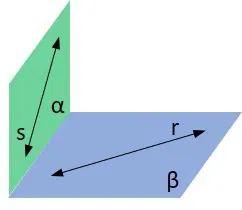
\includegraphics[width=3cm]{retas.png}
    \captionof{figure}{Axioma da reta.} % Isso coloca a legenda sem precisar de \begin{figure}
\end{center}
\end{block} 

\begin{block}{Axioma da escolha}
“Dada uma coleção de conjuntos não vazios, é possível escolher um elemento de cada conjunto, mesmo que a coleção seja infinita.”
\end{block}

\begin{block}{Axioma da escolha: Formalismo}
Dada uma família de conjuntos não vazios \(\{A_i\}_{i \in I}\), existe uma função de escolha
\[
f : I \to \bigcup_{i \in I} A_i
\]
tal que \(f(i) \in A_i\) para todo \(i \in I\).
\end{block}

\section{Quantificadores}

Na Matemática, muitas afirmações não tratam apenas de um elemento específico, mas de conjuntos inteiros de objetos. Quando dizemos, por exemplo, que “todo número par é divisível por 2” ou que “existe um número primo maior que 100”, estamos fazendo declarações que envolvem abrangência e existência. Para expressar esse tipo de ideia de forma precisa e sem ambiguidades, utilizamos os \textbf{quantificadores}.

Os quantificadores são símbolos e expressões da lógica matemática que indicam “para quais” ou “para quantos” elementos uma determinada proposição é válida. Eles permitem transformar frases da linguagem natural em sentenças formais, estruturadas e rigorosas. Os dois principais quantificadores são:

\begin{itemize}
    \item o \textbf{quantificador universal}, que expressa a ideia de “para todo”;
    \item o \textbf{quantificador existencial}, que expressa a ideia de “existe pelo menos um”.
\end{itemize}

Do ponto de vista intuitivo, os quantificadores ajudam a esclarecer o alcance de uma afirmação. Do ponto de vista do formalismo matemático, eles são essenciais para construir definições precisas, formular teoremas corretamente e elaborar demonstrações rigorosas. Uma pequena mudança no quantificador pode alterar completamente o significado de uma proposição.

Assim, compreender os quantificadores é dar um passo importante na transição da linguagem cotidiana para a linguagem formal da Matemática, desenvolvendo maior precisão no raciocínio e na escrita matemática.\subsection{Quantificador Existencial — “Existe”}

Ao afirmarmos que “existe” um elemento com determinada propriedade, estamos dizendo que pelo menos um objeto do conjunto considerado satisfaz a condição proposta. Não é necessário que todos satisfaçam a propriedade, nem que seja apenas um; basta que possamos indicar ao menos um exemplo válido.

Do ponto de vista do formalismo matemático, o quantificador existencial permite transformar afirmações intuitivas em enunciados rigorosos. Ele delimita claramente o conjunto no qual estamos procurando o elemento e explicita a propriedade que deve ser satisfeita. Em demonstrações, provar uma afirmação existencial geralmente exige a construção de um exemplo ou a prova de que tal elemento necessariamente deve existir.

\begin{block}{Definição}
A expressão \(\exists x \in A,\; P(x)\) significa que existe \textbf{pelo menos um} elemento \(x\) no conjunto \(A\) para o qual a proposição \(P(x)\) é verdadeira.
\end{block}

\begin{block}{Exemplo}
\[
\exists n \in \mathbb{Z},\; n^2 = 4
\]
(A proposição é verdadeira para \(n = 2\) e \(n = -2\).)
\end{block}



\subsection{Quantificador Existencial Único — “Existe um único”}

Em algumas situações, não basta garantir que exista um elemento com determinada propriedade; é necessário assegurar que ele seja o único. Essa distinção é fundamental em Matemática, pois muitas definições dependem da unicidade para evitar ambiguidades. Por exemplo, quando dizemos que uma equação tem solução única, estamos afirmando que há exatamente um valor que a satisfaz.

O quantificador existencial único combina duas ideias: existência e exclusividade. Formalmente, ele afirma que existe um elemento que satisfaz a propriedade e que nenhum outro elemento diferente dele possui essa mesma característica.

\begin{block}{Definição}
A expressão \(\exists! x \in A,\; P(x)\) significa que existe \textbf{um e somente um} elemento \(x\) no conjunto \(A\) para o qual a proposição \(P(x)\) é verdadeira.
\end{block}

\begin{block}{Exemplo}
\[
\exists! n \in \mathbb{N},\; n^2 = 1
\]
(A proposição é verdadeira apenas para \(n = 1\).)
\end{block}



\subsection{Quantificador Universal — “Para todo”}

O quantificador universal expressa generalidade. Quando afirmamos que uma propriedade vale “para todo” elemento de um conjunto, estamos garantindo que não há exceções dentro daquele domínio. Esse tipo de afirmação é comum em teoremas matemáticos, pois muitos resultados estabelecem propriedades válidas para todos os elementos de uma determinada classe.

No contexto do formalismo, o quantificador universal exige atenção especial ao conjunto considerado. Uma afirmação universal pode ser verdadeira em um conjunto e falsa em outro. Por isso, é essencial explicitar claramente o domínio sobre o qual a proposição está sendo feita.

\begin{block}{Definição}
A expressão \(\forall x \in A,\; P(x)\) significa que a proposição \(P(x)\) é verdadeira para \textbf{todos} os elementos \(x\) do conjunto \(A\).
\end{block}

O conceito de quantificação universal também aparece na definição de estruturas fundamentais, como o conjunto vazio. Observe que afirmar que um conjunto não possui elementos pode ser expresso formalmente por meio de uma proposição universal.

\begin{block}{Definição (Conjunto Vazio)}
Um conjunto \(A\) é chamado de \textbf{conjunto vazio} se, e somente se,
\[
\forall x,\; x \notin A.
\]
Denotamos o conjunto vazio por \(\varnothing\).
\end{block}\section{Definições}

Em Matemática, uma definição tem a função de estabelecer, com precisão e sem ambiguidades, o significado de um conceito. Diferentemente de descrições intuitivas, a definição matemática determina exatamente quais objetos pertencem a determinado conjunto e quais não pertencem. Isso é essencial para garantir rigor nos argumentos e clareza nas demonstrações.

Nesta seção, estudaremos a definição de círculo, analisando inicialmente sua interpretação geométrica e, em seguida, sua formulação algébrica no plano cartesiano.

\subsection{Definição de Círculo}

Intuitivamente, quando pensamos em um círculo, imaginamos uma figura redonda desenhada no plano. Entretanto, em Matemática, não basta uma descrição visual: é necessário caracterizar a figura por meio de uma propriedade precisa.

\begin{block}{Definição}
Seja \(C = (a,b) \in \mathbb{R}^2\) e seja \(r \in \mathbb{R}\) com \(r > 0\). Define-se o \textbf{círculo} de centro \(C\) e raio \(r\) como o conjunto
\[
\mathcal{C}(C,r) = \{\, (x,y) \in \mathbb{R}^2 \mid d\big((x,y),C\big) = r \,\},
\]
onde \(d\big((x,y),C\big) = \sqrt{(x-a)^2 + (y-b)^2}\) é a distância euclidiana entre o ponto \((x,y)\) e o centro \(C\). Equivalentemente, o círculo pode ser caracterizado pela equação
\[
(x-a)^2 + (y-b)^2 = r^2.
\]
\end{block}

Observe que a definição enfatiza duas ideias fundamentais:

\begin{itemize}
    \item O círculo é um \textbf{conjunto de pontos};
    \item Todos esses pontos estão à mesma distância do centro.
\end{itemize}

Essa distância constante é o que garante a forma geométrica do círculo. É importante destacar que o círculo corresponde apenas à “linha” que delimita a figura. A região interna pertence ao chamado \textbf{disco}, que é um conceito distinto.

\begin{figure}[H]
    \centering
    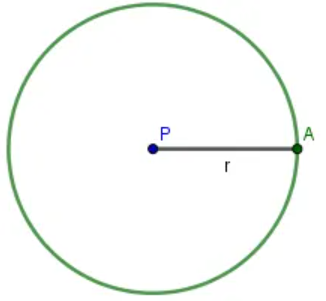
\includegraphics[width=4cm]{circulo2.png}
    \caption{Círculo de centro $C$ e raio $r$.} 
\end{figure}

\subsection{Explorando a definição de círculo}

Para expressar essa definição de maneira algébrica, utilizamos o plano cartesiano. Seja o centro do círculo o ponto \(C = (a,b) \in \mathbb{R}^2\) e seja \(r > 0\) o raio.

A distância entre um ponto qualquer \( (x,y) \) e o centro \( (a,b) \) é dada pela fórmula da distância no plano:

\[
d = \sqrt{(x-a)^2 + (y-b)^2}.
\]

Como todos os pontos do círculo estão exatamente à distância \(r\) do centro, impomos a condição:

\[
\sqrt{(x-a)^2 + (y-b)^2} = r.
\]

Elevando ambos os lados ao quadrado, obtemos a forma algébrica do círculo:

\[
(x-a)^2 + (y-b)^2 = r^2.
\]

Assim, o círculo de centro \(C\) e raio \(r\) pode ser descrito como o conjunto

\[
\mathcal{C}(C,r) = \{ (x,y) \in \mathbb{R}^2 \mid (x-a)^2 + (y-b)^2 = r^2 \}.
\]

Essa equação permite identificar, de maneira objetiva, se um ponto pertence ou não ao círculo.

\subsection{Aplicando a definição de círculo}

Vamos aplicar a definição para verificar a pertinência de alguns pontos.

Considere o círculo de centro \(C = (0,0)\) e raio \(r = 5\). Nesse caso, a equação do círculo é:

\[
x^2 + y^2 = 25.
\]

Desejamos verificar se os pontos abaixo pertencem ao círculo:

\[
P_1 = (3,4), \quad P_2 = (5,0), \quad P_3 = (2,2).
\]

\textbf{Critério:} Um ponto pertence ao círculo se, ao substituir suas coordenadas na equação, obtivermos \(25\).

\begin{itemize}
\item \(P_1 = (3,4)\):

\[
3^2 + 4^2 = 9 + 16 = 25.
\]

Como o resultado é igual a \(25\), o ponto pertence ao círculo.

\item \(P_2 = (5,0)\):

\[
5^2 + 0^2 = 25.
\]

Também pertence ao círculo.

\item \(P_3 = (2,2)\):

\[
2^2 + 2^2 = 4 + 4 = 8.
\]

Como \(8 < 25\), o ponto não pertence ao círculo. Ele está localizado no interior da circunferência.
\end{itemize}

Esse procedimento ilustra como a definição algébrica transforma uma ideia geométrica em um critério verificável, permitindo decidir com precisão matemática a pertença de pontos ao círculo.\section{Definição de Número Par e Número Ímpar}

As definições apresentadas nesta seção serão fundamentais para todo o desenvolvimento posterior do livro. Muitos resultados em Aritmética, Álgebra e Teoria dos Números dependem diretamente da caracterização formal de números pares e ímpares. Ao estabelecer essas definições com precisão, garantimos uma base rigorosa para demonstrações futuras, especialmente em argumentos que envolvem divisibilidade, propriedades algébricas e provas por contraposição ou contradição.

\begin{block}{Definição (Número Par)}
Um número inteiro \(n \in \mathbb{Z}\) é chamado de \textbf{par} se, e somente se, existe um inteiro \(k \in \mathbb{Z}\) tal que
\[
n = 2k.
\]
\end{block}

Essa definição expressa que um número é par exatamente quando é múltiplo de \(2\), isto é, quando é divisível por \(2\) sem deixar resto.

\begin{block}{Definição (Número Ímpar)}
Um número inteiro \(n \in \mathbb{Z}\) é chamado de \textbf{ímpar} se, e somente se, existe um inteiro \(k \in \mathbb{Z}\) tal que
\[
n = 2k + 1.
\]
\end{block}

Equivalente­mente, um número inteiro é ímpar quando não é divisível por \(2\), isto é, quando a divisão por \(2\) deixa resto igual a \(1\) ou \(-1\). Essas duas definições são mutuamente exclusivas e exaustivas no conjunto dos números inteiros: todo inteiro é ou par ou ímpar.
\subsection{Teorema Clássico — Soma de números pares}

\begin{block}{Teorema}
Se \(a\) e \(b\) são números inteiros pares, então \(a + b\) também é um número par.
\end{block}

\begin{block}{Prova}
Como \(a\) e \(b\) são pares, existem inteiros \(k\) e \(m\) tais que \(a = 2k\) e \(b = 2m\). Logo,
\[
a + b = 2k + 2m = 2(k+m),
\]
onde \(k+m\) é inteiro. Portanto, \(a + b\) é par.
\end{block}
\subsection{Exercícios — Provas com Números Pares}

\begin{block}{Exercício 1}
Prove que a soma de dois números inteiros ímpares é um número par.
\end{block}

\begin{block}{Exercício 2}
Prove que o produto de um número inteiro par por qualquer número inteiro é par.
\end{block}

\begin{block}{Exercício 3}
Mostre que, se \(n\) é um inteiro par, então \(n^2\) também é par.
\end{block}

\subsection{Respostas}

\begin{block}{Resposta do Exercício 1}
Sejam \(a\) e \(b\) números inteiros ímpares. Pela definição, existem inteiros \(k\) e \(m\) tais que \(a = 2k + 1\) e \(b = 2m + 1\). Logo,
\[
a + b = (2k + 1) + (2m + 1) = 2k + 2m + 2 = 2(k + m + 1).
\]
Como \(k + m + 1 \in \mathbb{Z}\), segue que \(a + b\) é múltiplo de \(2\). Portanto, a soma de dois números inteiros ímpares é um número par.
\end{block}

\begin{block}{Resposta do Exercício 2}
Seja \(a\) um número inteiro par. Então existe \(k \in \mathbb{Z}\) tal que \(a = 2k\). Seja \(b \in \mathbb{Z}\) arbitrário. Temos
\[
ab = (2k)b = 2(kb).
\]
Como \(kb \in \mathbb{Z}\), conclui-se que \(ab\) é múltiplo de \(2\). Logo, o produto de um número inteiro par por qualquer número inteiro é par.
\end{block}

\begin{block}{Resposta do Exercício 3}
Seja \(n\) um número inteiro par. Então existe \(k \in \mathbb{Z}\) tal que \(n = 2k\). Assim,
\[
n^2 = (2k)^2 = 4k^2 = 2(2k^2).
\]
Como \(2k^2 \in \mathbb{Z}\), segue que \(n^2\) é múltiplo de \(2\). Portanto, se \(n\) é par, então \(n^2\) também é par.
\end{block}\section{Lema}

No desenvolvimento de uma teoria matemática, muitas demonstrações são construídas em etapas. Frequentemente, antes de provar um resultado principal, é necessário estabelecer proposições intermediárias que organizam o raciocínio e simplificam a argumentação. Essas proposições recebem o nome de \textbf{lemas}.

\begin{block}{Definição}
Um \emph{lema} é uma proposição matemática demonstrável cuja principal finalidade é servir como \textbf{resultado auxiliar} na demonstração de um teorema ou de outro resultado mais abrangente. Embora possa possuir interesse próprio, sua função central é estruturar e viabilizar a prova de afirmações mais complexas.
\end{block}

Em termos metodológicos, o uso de lemas contribui para tornar as demonstrações mais claras, organizadas e modulares, permitindo que argumentos longos sejam divididos em partes logicamente independentes.

\begin{block}{Exemplo}
\textbf{Lema:} O quadrado de um número inteiro ímpar é ímpar.
\end{block}

Esse lema pode ser utilizado como passo auxiliar na demonstração de resultados mais gerais envolvendo propriedades de paridade. Por exemplo, ele é frequentemente empregado em provas por contraposição ou por contradição, como na demonstração de que, se \(n^2\) é par, então \(n\) é par. Assim, o lema funciona como uma ferramenta intermediária que simplifica e organiza a estrutura lógica de demonstrações mais amplas.
\subsection{Exemplo de Prova Utilizando Lemas}

Apresentamos a seguir um exemplo simples que ilustra como lemas podem ser utilizados para estruturar uma demonstração.

\begin{block}{Teorema}
Se \(n^2\) é um número inteiro par, então \(n\) é par.
\end{block}

Antes de demonstrar o teorema, estabelecemos um resultado auxiliar.

\begin{block}{Lema}
O quadrado de um número inteiro ímpar é ímpar.
\end{block}

\begin{block}{Prova do Lema}
Seja \(n\) um inteiro ímpar. Então existe \(k \in \mathbb{Z}\) tal que \(n = 2k + 1\). Logo,
\[
n^2 = (2k + 1)^2 = 4k^2 + 4k + 1 = 2(2k^2 + 2k) + 1.
\]
Como \(2k^2 + 2k \in \mathbb{Z}\), concluímos que \(n^2\) é da forma \(2m + 1\), com \(m \in \mathbb{Z}\). Portanto, \(n^2\) é ímpar.
\end{block}

\begin{block}{Prova do Teorema}
Suponha que \(n^2\) seja par. Demonstraremos que \(n\) também é par.

Procedemos por contraposição. Suponha que \(n\) seja ímpar. Pelo lema anterior, o quadrado de um número ímpar é ímpar. Logo, \(n^2\) seria ímpar.

Isso contradiz a hipótese de que \(n^2\) é par. Portanto, \(n\) não pode ser ímpar; consequentemente, \(n\) é par.
\end{block}

Observe que o lema permitiu isolar uma propriedade fundamental (o comportamento da paridade ao elevar ao quadrado), simplificando a demonstração do teorema principal e tornando o encadeamento lógico mais claro e organizado.
\section{Corolário}

No desenvolvimento de uma teoria matemática, muitos resultados surgem como consequências diretas de teoremas já estabelecidos. Quando uma proposição decorre de maneira imediata de um resultado anterior — isto é, quando sua demonstração exige apenas uma aplicação direta do que já foi provado — ela recebe o nome de \textbf{corolário}. O uso de corolários evidencia como um único teorema pode gerar diversas conclusões adicionais, ampliando seu alcance dentro da teoria.

\begin{block}{Definição}
Um \emph{corolário} é uma proposição que decorre de forma imediata de um teorema ou de um lema previamente demonstrado. Em geral, sua prova consiste apenas na aplicação direta do resultado anterior, não exigindo novos argumentos substanciais.
\end{block}

\begin{block}{Exemplo}
\textbf{Teorema:} Se \(n^2\) é um número inteiro par, então \(n\) é par.

\textbf{Corolário:} Se \(n\) é um número inteiro ímpar, então \(n^2\) é ímpar.
\end{block}

De fato, o corolário acima decorre imediatamente do teorema por contraposição lógica: se o quadrado de um número fosse par, então o número seria par; portanto, se o número é ímpar, seu quadrado não pode ser par, isto é, deve ser ímpar.

\subsection{Teorema e Corolário}

\begin{block}{Pergunta}
O corolário é um teorema?
\end{block}

\begin{block}{Resposta}
Sim. Um \emph{corolário} é, do ponto de vista lógico, um tipo particular de \emph{teorema}. A distinção entre eles é conceitual e didática: todo corolário é um teorema, pois é uma proposição demonstrável, mas nem todo teorema é um corolário. O termo “corolário” é utilizado quando se deseja enfatizar que o resultado é uma consequência direta e natural de outro já estabelecido.
\end{block}

Assim, a organização em teoremas, lemas e corolários não altera o valor lógico das proposições, mas contribui para estruturar o texto matemático de maneira clara e hierarquizada.

\section{Exercícios Complementares}


\section*{Exercícios}

\begin{enumerate}

\item Demonstre que a soma de dois números pares é sempre um número par.
\begin{block}{Resposta}
Sejam $a$ e $b$ dois números inteiros pares. Pela definição de número par, existem
$k,m \in \mathbb{Z}$ tais que $a = 2k$ e $b = 2m$. Assim, $ a+b = 2k + 2m = 2(k+m)$
onde $k+m \in \mathbb{Z}$. Logo, $a+b$ é par.
\end{block}


\item Demonstre que a soma de dois números ímpares é sempre um número par.
\begin{block}{Resposta}
Sejam $a$ e $b$ dois números inteiros ímpares. Existem $k,m \in \mathbb{Z}$ tais que
$a = 2k+1$ e $b = 2m+1$. Portanto,
$a+b = 2k+1 + 2m+1 = 2(k+m+1)$,
com $k+m+1 \in \mathbb{Z}$. Assim, a soma é par.
\end{block}
\item Demonstre que a soma de um número par com um número ímpar é sempre um número ímpar.

\item Prove que o produto de dois números inteiros ímpares é sempre ímpar.

\item Demonstre que o quadrado de qualquer número inteiro ímpar é ímpar.

\item Demonstre que, para qualquer inteiro \( n \), exatamente um dos números \( n \) ou \( n+1 \) é par.

\item Prove que, para todo inteiro \( n \), o número
\[
3n + 1
\]
possui paridade oposta à de \( n \).

\item Demonstre que a soma de três números inteiros consecutivos é sempre ímpar.
\newpage
\end{enumerate}


\begin{block}{3. Soma de um inteiro par com um inteiro ímpar}
Seja $a$ um inteiro par e $b$ um inteiro ímpar. Existem $k,m \in \mathbb{Z}$ tais que
$a = 2k$ e $b = 2m+1$. Logo,
\[
a+b = 2k + 2m + 1 = 2(k+m)+1,
\]
onde $k+m \in \mathbb{Z}$. Portanto, a soma é ímpar.
\end{block}

\begin{block}{4. Produto de dois inteiros ímpares}
Sejam $a$ e $b$ dois inteiros ímpares. Existem $k,m \in \mathbb{Z}$ tais que
$a = 2k+1$ e $b = 2m+1$. O produto é
\[
ab = (2k+1)(2m+1) = 2(2km+k+m)+1,
\]
com $2km+k+m \in \mathbb{Z}$. Logo, $ab$ é ímpar.
\end{block}

\begin{block}{5. Quadrado de um inteiro ímpar}
Seja $n$ um inteiro ímpar. Existe $k \in \mathbb{Z}$ tal que $n = 2k+1$. Assim,
\[
n^2 = (2k+1)^2 = 2(2k^2+2k)+1,
\]
onde $2k^2+2k \in \mathbb{Z}$. Portanto, o quadrado de um inteiro ímpar é ímpar.
\end{block}

\begin{block}{6. Paridade de $n$ e $n+1$}
Seja $n \in \mathbb{Z}$. Se $n$ é par, então $n=2k$ e $n+1=2k+1$, que é ímpar.
Se $n$ é ímpar, então $n=2k+1$ e $n+1=2(k+1)$, que é par.
Assim, exatamente um dos números $n$ ou $n+1$ é par.
\end{block}

\begin{block}{7. Paridade de $3n+1$}
Seja $n \in \mathbb{Z}$. Se $n=2k$, então
\[
3n+1 = 6k+1 = 2(3k)+1,
\]
que é ímpar. Se $n=2k+1$, então
\[
3n+1 = 6k+4 = 2(3k+2),
\]
que é par. Logo, $3n+1$ tem paridade oposta à de $n$.
\end{block}

\begin{block}{8. Soma de três inteiros consecutivos}
Sejam três inteiros consecutivos $n-1$, $n$ e $n+1$. A soma é
\[
(n-1)+n+(n+1)=3n.
\]
Se $n$ é par, então $3n$ é par; se $n$ é ímpar, então $3n$ é ímpar.
Em ambos os casos, a soma dos três inteiros consecutivos é ímpar.
\end{block}
\section*{Instruções}

\begin{block}{Utilize a definição formal de divisibilidade}
Sejam $a,b \in \mathbb{Z}$, com $b \neq 0$. Dizemos que $b$ divide $a$ se existe
$k \in \mathbb{Z}$ tal que
\[
a = bk.
\]
Neste caso, escrevemos $b \mid a$.
\end{block}

Justifique rigorosamente todas as afirmações utilizando apenas definições formais
e propriedades dos números inteiros.
% =======================
% EXERCÍCIOS (SEM RESPOSTA)
% =======================

\section*{Exercícios}

\begin{enumerate}

\item Demonstre que, se $a \mid b$ e $a \mid c$, então $a \mid (b+c)$.

\item Demonstre que, se $a \mid b$, então $a \mid (-b)$.

\item Prove que, se $a \mid b$ e $b \mid c$, então $a \mid c$.



\end{enumerate}

\newpage

% =======================
% GABARITO
% =======================

\section*{Gabarito — Respostas}
\begin{block}{1. Soma preserva divisibilidade}
Suponha que $a \mid b$ e $a \mid c$. Pela definição de divisibilidade, existem
inteiros $k,m \in \mathbb{Z}$ tais que $b = ak$ e $c = am$. Somando essas
igualdades, obtemos $b + c = ak + am = a(k+m)$
Como $k+m \in \mathbb{Z}$, segue diretamente da definição que
$a \mid (b+c)$, concluindo a demonstração.
\end{block}

\begin{block}{2. Divisibilidade pelo oposto}
Suponha que $a \mid b$. Então, pela definição de divisibilidade, existe
$k \in \mathbb{Z}$ tal que $b = ak$. Multiplicando ambos os lados da igualdade
por $-1$, temos
$-b = a(-k).$
Como $-k \in \mathbb{Z}$, conclui-se que $a \mid (-b)$, conforme a definição
formal de divisibilidade.
\end{block}

\begin{block}{3. Transitividade da divisibilidade}
Suponha que $a \mid b$ e $b \mid c$. Pela definição, existem inteiros
$k,m \in \mathbb{Z}$ tais que $b = ak$ e $c = bm$. Substituindo a expressão
de $b$ na igualdade que define $c$, obtemos
$
c = (ak)m = a(km).
$
Como $km \in \mathbb{Z}$, segue pela definição de divisibilidade que
$a \mid c$, o que demonstra a transitividade da relação de divisibilidade.
\end{block}
% =======================
% Capítulo 1: Proposições e Conectivos
% =======================
\chapter{Proposições e Conectivos Lógicos}

A Lógica é a base formal de toda a Matemática. Antes de desenvolver demonstrações, construir definições ou estabelecer teoremas, é necessário compreender o que constitui uma afirmação matemática e como diferentes afirmações podem ser combinadas. Neste capítulo, estudaremos o conceito de proposição e os conectivos lógicos que permitem estruturar argumentos de maneira rigorosa.

\section{Proposição}

Em Matemática, trabalhamos com afirmações cujo valor de verdade pode ser determinado de forma objetiva. Essas afirmações são os elementos fundamentais do raciocínio lógico e recebem o nome de proposições.

\begin{block}{Definição}
Uma \textbf{proposição} é uma sentença declarativa à qual se pode atribuir exatamente um valor lógico: \textbf{verdadeiro} (V) ou \textbf{falso} (F), mas não ambos simultaneamente.
\end{block}

A exigência de que a sentença seja declarativa é essencial. Uma proposição deve afirmar algo sobre determinado objeto, propriedade ou relação. Além disso, seu valor lógico precisa estar bem definido, independentemente de opiniões pessoais ou ambiguidades linguísticas.

\begin{block}{Exemplos}
\begin{itemize}
    \item “$2 + 2 = 4$” — proposição verdadeira, pois a igualdade é válida no conjunto dos números reais.
    \item “$5$ é um número par” — proposição falsa, pois $5$ não é divisível por $2$.
    \item “Glifosato é um herbicida” — proposição verdadeira, pois descreve corretamente uma propriedade da substância.
\end{itemize}
\end{block}

Observe que, em todos os casos acima, é possível decidir objetivamente se a afirmação é verdadeira ou falsa.

\begin{block}{Não Exemplos}
As sentenças a seguir \textbf{não} são proposições:
\begin{itemize}
    \item “Qual é a sua idade?” — trata-se de uma pergunta, não de uma afirmação.
    \item “Estude para a prova!” — trata-se de uma ordem ou comando.
\end{itemize}
\end{block}

Perguntas, ordens, exclamações e sentenças abertas (como “$x > 3$”, sem especificar o valor de $x$) não são proposições, pois não possuem valor lógico determinado enquanto não forem completadas ou contextualizadas adequadamente.

Compreender o conceito de proposição é fundamental, pois todo o desenvolvimento da Lógica Matemática — incluindo conectivos, quantificadores e demonstrações — baseia-se na manipulação rigorosa de proposições e de seus valores de verdade.
\section{Conjunção e Disjunção}

Uma vez compreendido o conceito de proposição, o próximo passo consiste em estudar as formas pelas quais proposições podem ser combinadas para formar novas afirmações. Essas combinações são realizadas por meio dos chamados \textbf{conectivos lógicos}. Entre os conectivos fundamentais destacam-se a \emph{conjunção} e a \emph{disjunção}, que formalizam, respectivamente, as ideias de “e” e “ou” na linguagem matemática.

\begin{block}{Conectivos \textbf{E} ($\land$) e \textbf{OU} ($\lor$)}
Sejam \(P\) e \(Q\) proposições.

\begin{itemize}
    \item A \textbf{conjunção} \(P \land Q\) é a proposição que afirma simultaneamente \(P\) e \(Q\). Ela é verdadeira se, e somente se, \textbf{ambas} as proposições \(P\) e \(Q\) forem verdadeiras.
    
    \item A \textbf{disjunção} \(P \lor Q\) é a proposição que afirma que pelo menos uma entre \(P\) e \(Q\) é verdadeira. Ela é verdadeira se \textbf{ao menos uma} das proposições for verdadeira, podendo ambas serem verdadeiras.
\end{itemize}
\end{block}

É importante destacar que, em Lógica Matemática, o conectivo “ou” é utilizado no sentido inclusivo. Assim, a proposição \(P \lor Q\) é verdadeira quando \(P\) é verdadeira, quando \(Q\) é verdadeira ou quando ambas são verdadeiras.

\subsection*{Propriedades Fundamentais}

Assim como as operações aritméticas possuem propriedades estruturais, os conectivos lógicos também obedecem a leis formais que garantem coerência e flexibilidade na manipulação de proposições.

\begin{block}{Propriedades Algébricas da Conjunção e da Disjunção}
Para quaisquer proposições \(P\), \(Q\) e \(R\), valem as seguintes equivalências lógicas:

\begin{itemize}
    \item \textbf{Comutatividade}
    \[
        P \land Q \equiv Q \land P, 
        \qquad
        P \lor Q \equiv Q \lor P.
    \]
    A ordem das proposições não altera o valor lógico da conjunção ou da disjunção.

    \item \textbf{Associatividade}
    \[
        (P \land Q) \land R \equiv P \land (Q \land R), 
        \qquad
        (P \lor Q) \lor R \equiv P \lor (Q \lor R).
    \]
    O modo como as proposições são agrupadas não interfere no resultado lógico.

    \item \textbf{Idempotência}
    \[
        P \land P \equiv P, 
        \qquad 
        P \lor P \equiv P.
    \]
    Repetir a mesma proposição em uma conjunção ou disjunção não altera seu valor lógico.
\end{itemize}
\end{block}

Essas propriedades desempenham papel fundamental na simplificação de expressões lógicas e na construção de demonstrações formais, funcionando de maneira análoga às propriedades estruturais das operações algébricas.
\section{Tabelas-Verdade}

Na Lógica Proposicional, uma questão central consiste em determinar o valor lógico de uma fórmula composta a partir dos valores de verdade de suas proposições elementares. Para esse fim, um dos métodos mais fundamentais e sistemáticos é o \textbf{método da tabela-verdade}. Trata-se de um procedimento formal que permite analisar completamente o comportamento lógico de uma expressão.

\begin{block}{Ideia Geral}
A tabela-verdade é um instrumento que organiza, de maneira sistemática, todas as possíveis atribuições de valores lógicos às proposições simples envolvidas em uma fórmula, permitindo calcular, em cada caso, o valor lógico da expressão composta.
\end{block}

\begin{block}{Definição}
A \textbf{tabela-verdade} é um método \emph{exaustivo} de verificação lógica que consiste em listar todas as possíveis valorações das proposições atômicas de uma fórmula \(A\) e determinar, para cada uma delas, o valor lógico resultante da fórmula.
\end{block}

Diz-se que o método é exaustivo porque considera todas as combinações possíveis de valores verdadeiros (V) e falsos (F). Se uma fórmula contém \(n\) proposições atômicas distintas, sua tabela-verdade possuirá \(2^n\) linhas, correspondendo a todas as possíveis atribuições de valores lógicos.

\begin{figure}[h]
    \centering
    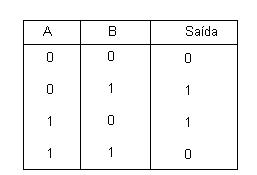
\includegraphics[width=0.4\linewidth]{tabela_verdade1.jpeg}
    \caption{Exemplo de tabela-verdade.}
\end{figure}

\begin{block}{Estrutura da Tabela}
Uma tabela-verdade é organizada da seguinte forma:
\begin{itemize}
    \item Cada proposição atômica (ou átomo lógico) recebe uma coluna própria.
    \item As colunas correspondentes aos átomos aparecem à esquerda.
    \item Colunas intermediárias podem ser incluídas para registrar o valor de subfórmulas.
    \item A coluna mais à direita contém o valor lógico da fórmula principal.
\end{itemize}
\end{block}

O uso de tabelas-verdade permite verificar propriedades importantes, como se uma fórmula é uma tautologia (sempre verdadeira), uma contradição (sempre falsa) ou uma contingência (ora verdadeira, ora falsa). Dessa forma, esse método constitui uma ferramenta essencial para a análise formal de argumentos e para a validação de raciocínios lógicos.
\section{Exaustividade e Complexidade}

\begin{block}{Importante Observação}
Ao final da construção da tabela da verdade, \textbf{todas as possíveis valorações da fórmula $A$ são consideradas}.
\end{block}

\begin{block}{Número de Valorações}
Se uma fórmula contém $n$ átomos, então o número de valorações possíveis é:
\[
2^n
\]
Consequentemente, a tabela da verdade terá exatamente $2^n$ linhas.
\end{block}
\section{Tabelas dos Conectivos}

Para construir tabelas-verdade de fórmulas mais complexas, é indispensável conhecer previamente o comportamento lógico de cada conectivo. As tabelas a seguir apresentam, de maneira formal, como os valores de verdade são determinados para a negação, a conjunção e a disjunção.

\subsection*{Negação ($\neg$)}

A negação é um conectivo unário, isto é, atua sobre uma única proposição. Seu efeito é inverter o valor lógico da proposição original.

\begin{block}{Tabela da Negação}
\[
\begin{array}{c|c}
p & \neg p \\ \hline
V & F \\
F & V
\end{array}
\]
\end{block}

Assim, se \(p\) é verdadeira, então \(\neg p\) é falsa; se \(p\) é falsa, então \(\neg p\) é verdadeira.

\subsection*{Conjunção ($\land$)}

A conjunção expressa a ideia de simultaneidade lógica: a proposição composta \(p \land q\) afirma que \(p\) e \(q\) são ambas verdadeiras.

\begin{block}{Tabela da Conjunção}
\[
\begin{array}{c|c|c}
p & q & p \land q \\ \hline
V & V & V \\
V & F & F \\
F & V & F \\
F & F & F
\end{array}
\]
\end{block}

Observa-se que a conjunção somente é verdadeira quando as duas proposições componentes são verdadeiras simultaneamente.

\subsection*{Disjunção ($\lor$)}

A disjunção, na lógica matemática, é entendida no sentido inclusivo. A proposição \(p \lor q\) é verdadeira sempre que pelo menos uma das proposições for verdadeira.

\begin{block}{Tabela da Disjunção}
\[
\begin{array}{c|c|c}
p & q & p \lor q \\ \hline
V & V & V \\
V & F & V \\
F & V & V \\
F & F & F
\end{array}
\]
\end{block}

Note que a disjunção é falsa apenas quando ambas as proposições são falsas.

\section{Exemplo Completo}

A seguir, construiremos a tabela-verdade da fórmula
\[
(P \lor Q) \land (\neg P \lor \neg Q).
\]

O procedimento consiste em:
\begin{itemize}
    \item listar todas as possíveis combinações de valores para \(P\) e \(Q\);
    \item calcular os valores das negações;
    \item determinar os valores das subfórmulas intermediárias;
    \item finalmente, calcular o valor da fórmula principal.
\end{itemize}

\[
\begin{array}{c|c|c|c|c|c|c}
P & Q & \neg P & \neg Q & P \lor Q & \neg P \lor \neg Q & (P \lor Q) \land (\neg P \lor \neg Q) \\ \hline
V & V & F & F & V & F & F \\
V & F & F & V & V & V & V \\
F & V & V & F & V & V & V \\
F & F & V & V & F & V & F
\end{array}
\]

Observa-se que a fórmula é verdadeira apenas quando exatamente uma das proposições \(P\) ou \(Q\) é verdadeira. Esse tipo de análise evidencia como a tabela-verdade permite compreender com precisão o comportamento lógico de fórmulas compostas.
\section{Exercícios}

\begin{block}{Exercício 1}
Construa a tabela da verdade para a fórmula:
\[
(P \land Q) \lor \neg Q
\]
\end{block}

\begin{block}{Resposta do Exercício 1}

Para construir a tabela, listamos inicialmente todas as combinações possíveis dos valores de \(P\) e \(Q\). Em seguida, calculamos as colunas intermediárias \(P \land Q\) e \(\neg Q\), finalizando com a fórmula principal.

\[
\begin{array}{c|c|c|c|c}
P & Q & P \land Q & \neg Q & (P \land Q) \lor \neg Q \\ \hline
V & V & V & F & V \\
V & F & F & V & V \\
F & V & F & F & F \\
F & F & F & V & V
\end{array}
\]

Observa-se que a fórmula é verdadeira em três das quatro linhas e falsa apenas quando \(P\) é falsa e \(Q\) é verdadeira. Logo, trata-se de uma \emph{contingência}, pois não é sempre verdadeira nem sempre falsa.
\end{block}

\begin{block}{Exercício 2}
Faça a tabela da verdade para:
\[
(P \lor Q) \land (\neg P \land \neg Q)
\]
Observe se a fórmula assume valor verdadeiro em todas as linhas, em nenhuma, ou apenas em algumas.
\end{block}

\begin{block}{Resposta do Exercício 2}

Procedemos de maneira análoga, construindo as colunas intermediárias necessárias.

\[
\begin{array}{c|c|c|c|c|c|c}
P & Q & P \lor Q & \neg P & \neg Q & \neg P \land \neg Q & (P \lor Q) \land (\neg P \land \neg Q) \\ \hline
V & V & V & F & F & F & F \\
V & F & V & F & V & F & F \\
F & V & V & V & F & F & F \\
F & F & F & V & V & V & F
\end{array}
\]

Verifica-se que a fórmula é falsa em todas as linhas da tabela. Portanto, trata-se de uma \emph{contradição}, isto é, uma proposição que nunca assume valor verdadeiro.

Essa análise ilustra como a tabela-verdade permite classificar formalmente uma fórmula como tautologia, contradição ou contingência.
\end{block}

\begin{block}{Exercício 3}
Construa a tabela-verdade da fórmula:
\[
\neg(P \land Q)
\]
e compare o resultado com a fórmula \(\neg P \lor \neg Q\).
\end{block}

\begin{block}{Resposta do Exercício 3}

Construímos inicialmente a tabela para \(\neg(P \land Q)\).

\[
\begin{array}{c|c|c|c}
P & Q & P \land Q & \neg(P \land Q) \\ \hline
V & V & V & F \\
V & F & F & V \\
F & V & F & V \\
F & F & F & V
\end{array}
\]

Agora, construímos a tabela para \(\neg P \lor \neg Q\).

\[
\begin{array}{c|c|c|c|c}
P & Q & \neg P & \neg Q & \neg P \lor \neg Q \\ \hline
V & V & F & F & F \\
V & F & F & V & V \\
F & V & V & F & V \\
F & F & V & V & V
\end{array}
\]

Observa-se que as colunas finais são idênticas. Portanto,
\[
\neg(P \land Q) \equiv \neg P \lor \neg Q,
\]
o que confirma uma das Leis de De Morgan.
\end{block}

\begin{block}{Exercício 4}
Construa a tabela-verdade da fórmula:
\[
(P \lor Q) \lor \neg P.
\]
Classifique a fórmula como tautologia, contradição ou contingência.
\end{block}

\begin{block}{Resposta do Exercício 4}

\[
\begin{array}{c|c|c|c|c}
P & Q & P \lor Q & \neg P & (P \lor Q) \lor \neg P \\ \hline
V & V & V & F & V \\
V & F & V & F & V \\
F & V & V & V & V \\
F & F & F & V & V
\end{array}
\]

Como a fórmula assume valor verdadeiro em todas as linhas, concluímos que se trata de uma \textbf{tautologia}.
\end{block}

\begin{block}{Exercício 5}
Construa a tabela-verdade da fórmula:
\[
(P \land \neg P) \lor Q.
\]
Determine sua classificação lógica.
\end{block}

\begin{block}{Resposta do Exercício 5}

\[
\begin{array}{c|c|c|c|c|c}
P & Q & \neg P & P \land \neg P & (P \land \neg P) \lor Q \\ \hline
V & V & F & F & V \\
V & F & F & F & F \\
F & V & V & F & V \\
F & F & V & F & F
\end{array}
\]

Note que \(P \land \neg P\) é sempre falso, pois uma proposição não pode ser simultaneamente verdadeira e falsa. Assim, a fórmula reduz-se logicamente a \(Q\). Como assume valor verdadeiro em algumas linhas e falso em outras, trata-se de uma \textbf{contingência}.
\end{block}




% =======================
% Capítulo 3: Implicação Lógica
% =======================
\chapter{Implicação Lógica}

\section{Contexto Histórico}

\begin{block}{Origens}
O conceito de implicação lógica tem origem na lógica aristotélica, mas assume sua forma moderna a partir do século XIX com o desenvolvimento da lógica simbólica por matemáticos como George Boole, Gottlob Frege e Bertrand Russell.
\end{block}

\section{Definição e Intuição}

\begin{block}{Ideia Intuitiva}
A expressão \(P \Rightarrow Q\) deve ser lida como: “Se \(P\) é verdadeiro, então \(Q\) é verdadeiro”.
\end{block}

\begin{block}{Definição Formal}
Sejam \(P\) e \(Q\) proposições. A implicação \(P \Rightarrow Q\) é falsa apenas quando \(P\) é verdadeira e \(Q\) é falsa. Em todos os demais casos, é verdadeira.
\end{block}

\begin{block}{Tabela-Verdade da Implicação}
\[
\begin{array}{c|c|c}
P & Q & P \Rightarrow Q \\ \hline
V & V & V \\
V & F & F \\
F & V & V \\
F & F & V
\end{array}
\]
\end{block}

\section{Propriedades e Uso com Quantificadores}

\begin{block}{Propriedade Fundamental}
Se \(P\) é falsa, então a implicação \(P \Rightarrow Q\) é verdadeira para qualquer proposição \(Q\).
\end{block}

\begin{block}{Uso em Definições}
A implicação aparece naturalmente em definições matemáticas, como na definição de subconjunto:
\[
A \subseteq B \;\Longleftrightarrow\; \forall x,\; (x \in A \Rightarrow x \in B).
\]
\end{block}

\section{Volta da Implicação}

\begin{block}{Definição}
A \textbf{volta} (ou conversa) da implicação \(P \Rightarrow Q\) é a proposição \(Q \Rightarrow P\).
\end{block}

\begin{block}{Observação}
Em geral, \(P \Rightarrow Q\) não implica \(Q \Rightarrow P\). A implicação não é reversível.
\end{block}

\begin{block}{Exemplo}
\begin{itemize}
    \item Implicação: Se um número é múltiplo de 4, então é par. (Verdadeira)
    \item Volta: Se um número é par, então é múltiplo de 4. (Falsa)
\end{itemize}
\end{block}

\section{Análise Formal da Hipótese}

\begin{block}{Caracterização Lógica}
Para quaisquer proposições \(P\) e \(Q\):
\[
P \Rightarrow Q \text{ é falsa} \iff (P = V) \land (Q = F).
\]
Equivalentemente,
\[
\forall P\,\forall Q,\; (P = F) \;\Rightarrow\; (P \Rightarrow Q = V).
\]
Ou seja, quando a hipótese é falsa, a implicação é verdadeira, independentemente de \(Q\).
\end{block}

% =======================
% Capítulo 4: Bicondicional
% =======================
\chapter{Bicondicional}

\begin{block}{Definição}
A proposição \(P \Leftrightarrow Q\) (lê-se “\(P\) se e somente se \(Q\)”) é verdadeira quando \(P\) e \(Q\) têm o mesmo valor lógico (ambas verdadeiras ou ambas falsas).
\end{block}

\begin{block}{Tabela-Verdade}
\[
\begin{array}{c|c|c}
P & Q & P \Leftrightarrow Q \\ \hline
V & V & V \\
V & F & F \\
F & V & F \\
F & F & V
\end{array}
\]
\end{block}

\begin{block}{Interpretação}
O bicondicional só falha quando os valores de \(P\) e \(Q\) são diferentes.
\end{block}

% =======================
% Capítulo 5: Teoria dos Conjuntos (opcional, baseado nos slides)
% =======================
\chapter{Noções de Teoria dos Conjuntos}

\section{Definição de Conjunto}

\begin{block}{Conjunto}
Um \textbf{conjunto} é uma coleção bem definida de elementos distintos, denotada por uma letra maiúscula.
\end{block}

Seja \(A\) um conjunto e \(x\) um elemento:
\[
x \in A \quad \text{(x pertence a A)}, \qquad
x \notin A \quad \text{(x não pertence a A)}.
\]

\begin{block}{Definição por Extensão}
Listagem explícita dos elementos:
\[
A = \{a_1, a_2, \dots, a_n\}.
\]
\end{block}

\begin{block}{Definição por Compreensão}
Caracterização por uma propriedade lógica:
\[
A = \{\, x \in U \mid P(x) \,\}.
\]
\end{block}

\section{Conjunto Vazio}

\begin{block}{Definição}
O \textbf{conjunto vazio}, denotado por \(\varnothing\) ou \(\emptyset\), é o conjunto que não possui nenhum elemento.
Formalmente:
\[
\varnothing = \{\, x \mid x \neq x \,\}.
\]
\end{block}

\begin{block}{Exemplos}
\[
\begin{aligned}
A_1 &= \{\, x \in \mathbb{R} \mid x \neq x \,\} \\
A_2 &= \{\, (x,y) \in \mathbb{R}^2 \mid x+y=1 \text{ e } x+y=2 \,\} \\
A_3 &= \{\, x \in \mathbb{N} \mid x < 0 \,\} \\
A_4 &= \{\, x \in \mathbb{R} \mid x^2 < 0 \,\}
\end{aligned}
\]
Todos são vazios, pois as condições são impossíveis.
\end{block}

\section{Cardinalidade}

\begin{block}{Definição}
A \textbf{cardinalidade} de um conjunto \(A\), denotada por \(|A|\), é o número de elementos de \(A\).
\end{block}

\begin{block}{Conjuntos Finitos e Infinitos}
\begin{itemize}
    \item \(A = \{1,3,5,7\}\) é finito, \(|A|=4\).
    \item \(\mathbb{N} = \{0,1,2,3,\dots\}\) é infinito.
\end{itemize}
\end{block}

\section{Pertinência e Continência}

\begin{block}{Pertinência (\(x \in A\))}
Relação entre elemento e conjunto.
\end{block}

\begin{block}{Continência (\(A \subseteq B\))}
Relação entre conjuntos: \(A \subseteq B\) significa que todo elemento de \(A\) também pertence a \(B\):
\[
A \subseteq B \iff \forall x,\; (x \in A \Rightarrow x \in B).
\]
\end{block}

\begin{observacao}
A pertinência relaciona \textbf{elemento–conjunto}, enquanto a continência relaciona \textbf{conjunto–conjunto}. São relações de naturezas distintas.
\end{observacao}

\end{document}
